\documentclass[journal]{IEEEtran}

\usepackage{graphicx}
\usepackage{amsmath}


\begin{document}

\title{An Acquisition system for CMOS imagers with a genuine 10 Gbit/s bandwidth}

\author{
C. Gu\'erin, R. Barbier, J. Marhoug, W. Tromeur, J. Houles, Q. T. Doan, A. Dominjon, T. Cajgfinger
     
\thanks{C. Gu\'erin is with the Institut de Physique Nucl\'eaire de Lyon, France (telephone: +33 4 12 34 56 78, e-mail: c.guerin@abc.ef.fr).}

\thanks{R. Barbier is with the Institut de Physique Nucl\'eaire de Lyon, France (telephone: +33 4 12 34 56 78, e-mail: r.barbier@abc.ef.fr).}
}

\markboth{Nuclear Science Symposium and Medical Imaging Conference (NSS/MIC), 2011 IEEE} {C. Gu\'erin \textit{et al.}: An Acquisition system for CMOS imagers with a genuine 10 Gbit/s bandwidth}

\maketitle

\begin{abstract}
This paper presents a high data throughput acquisition system for pixel detector readout such as CMOS imagers ...
\end{abstract}

\begin{IEEEkeywords}
CMOS image sensors, adaptive optics, data acquisition, image resolution, nanophotonics.
\end{IEEEkeywords}


\section{Introduction}
\label{sec:intro}

\IEEEPARstart{T}{he} CMOS Image Sensors (CIS) are able to provide highdefinition images at an ultra-fast frame rate, thanks to the reduction of the grid size ...

\section{Synoptic of the data acquisition system}
\label{sec:synoptic}

The imaging system is composed of 3 main blocks\cite{bib_remi2011} and within the S/N ratios at different frame rate as shown in the Table \ref{tab:data} ...

\begin{table}[!htb]
\centering
	\caption{S/N ratios.}
	\label{tab:data} 
	\begin{tabular}{ccc}
		\hline
		Frame rate	& S/N ratio\\
		\hline
		125	& 2.0\\
		250	& 1.5\\
		500	& 1.1\\
		\hline
	\end{tabular}
\end{table}

\section{Daq boards}
\label{sec:daq}
The DAQ board has been designed ...


\section{Software}
\label{sec:soft}

\subsection{The software platform}
The computer is in charge of data reception ...
\subsection{Implementation, optimization and performances}
When working at 500 frames per second, we obtained image as shown in the Figure \ref{fig:microlens} ...

\begin{figure}[!htb]
\centering
	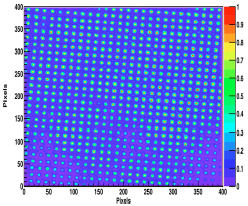
\includegraphics[width=0.5\linewidth]{microlens.png}
	\caption{Image capture of a microlens 400x400 pixels.}
	\label{fig:microlens}
\end{figure}


\section{Conclusion}
We presented in this paper an acquisition system for CMOS imager with a true 10 Gbit/s bandwidth ...


\appendices
\section{Tracking algorithm}
Tracking algorith was implemented for more than 2000 targets ...

\section{Target list visualization}
Trajectory of bacteria was drawn ...


\section*{Acknowledgment}
The LUSIPHER Project is supported by grants from Institut National de Physique Nucl\'eaire et de Physique


\bibliographystyle{ieeetr} 
\bibliography{biblio}



\begin{IEEEbiography}[{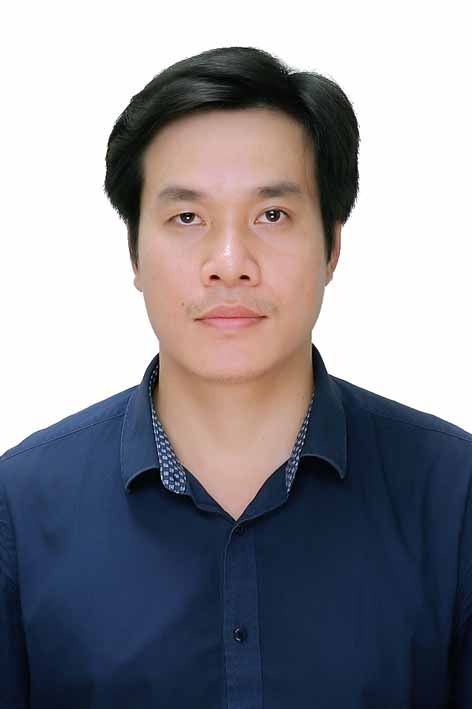
\includegraphics[width=0.5in, keepaspectratio]{tuyen.jpg}}]{Q. T. Doan}
Ph.D in nuclear physics, working at IPNL since ...
\end{IEEEbiography}

\begin{IEEEbiographynophoto}{Remi Barbier}
Ph.D in nuclear physics, working at IPNL since ...
\end{IEEEbiographynophoto}

\begin{IEEEbiographynophoto}{C. Gu\'erin}
Engineer, working at IPNL since ....
\end{IEEEbiographynophoto}

\end{document}


